%
% $RCSfile: cybernetics_oriented_language.tex,v $
%
% Copyright (c) 2001-2004. Christian Heller. All rights reserved.
%
% No copying, altering, distribution or any other actions concerning this
% document, except after explicit permission by the author!
% At some later point in time, this document is planned to be put under
% the GNU FDL license. For now, _everything_ is _restricted_ by the author.
%
% http://www.cybop.net
% - Cybernetics Oriented Programming -
%
% http://www.resmedicinae.org
% - Information in Medicine -
%
% @author Christian Heller <christian.heller@tuxtax.de>
%

\section{Cybernetics Oriented Language}
\label{cybernetics_oriented_language_heading}

The introduced \emph{Cybernetics Oriented Language} (CYBOL) is based on the
principles of \emph{Human Thinking} as described in section \ref{human_thinking_heading}.
These principles and further concepts behind are summarized by the name
\emph{Cybernetics Oriented Programming} (CYBOP) (figure \ref{cybop_figure}).
They form the semantics of CYBOL. Its syntax is determined by the \emph{Extensible
Markup Language} (XML) standard and accordingly easy. It is rich enough to express
models based upon the three kinds of abstraction: \emph{Discrimination},
\emph{Categorization} and \emph{Composition} as well as meta information of a
\emph{Whole} about its \emph{Parts}.

\begin{figure}[ht]
    \begin{center}
        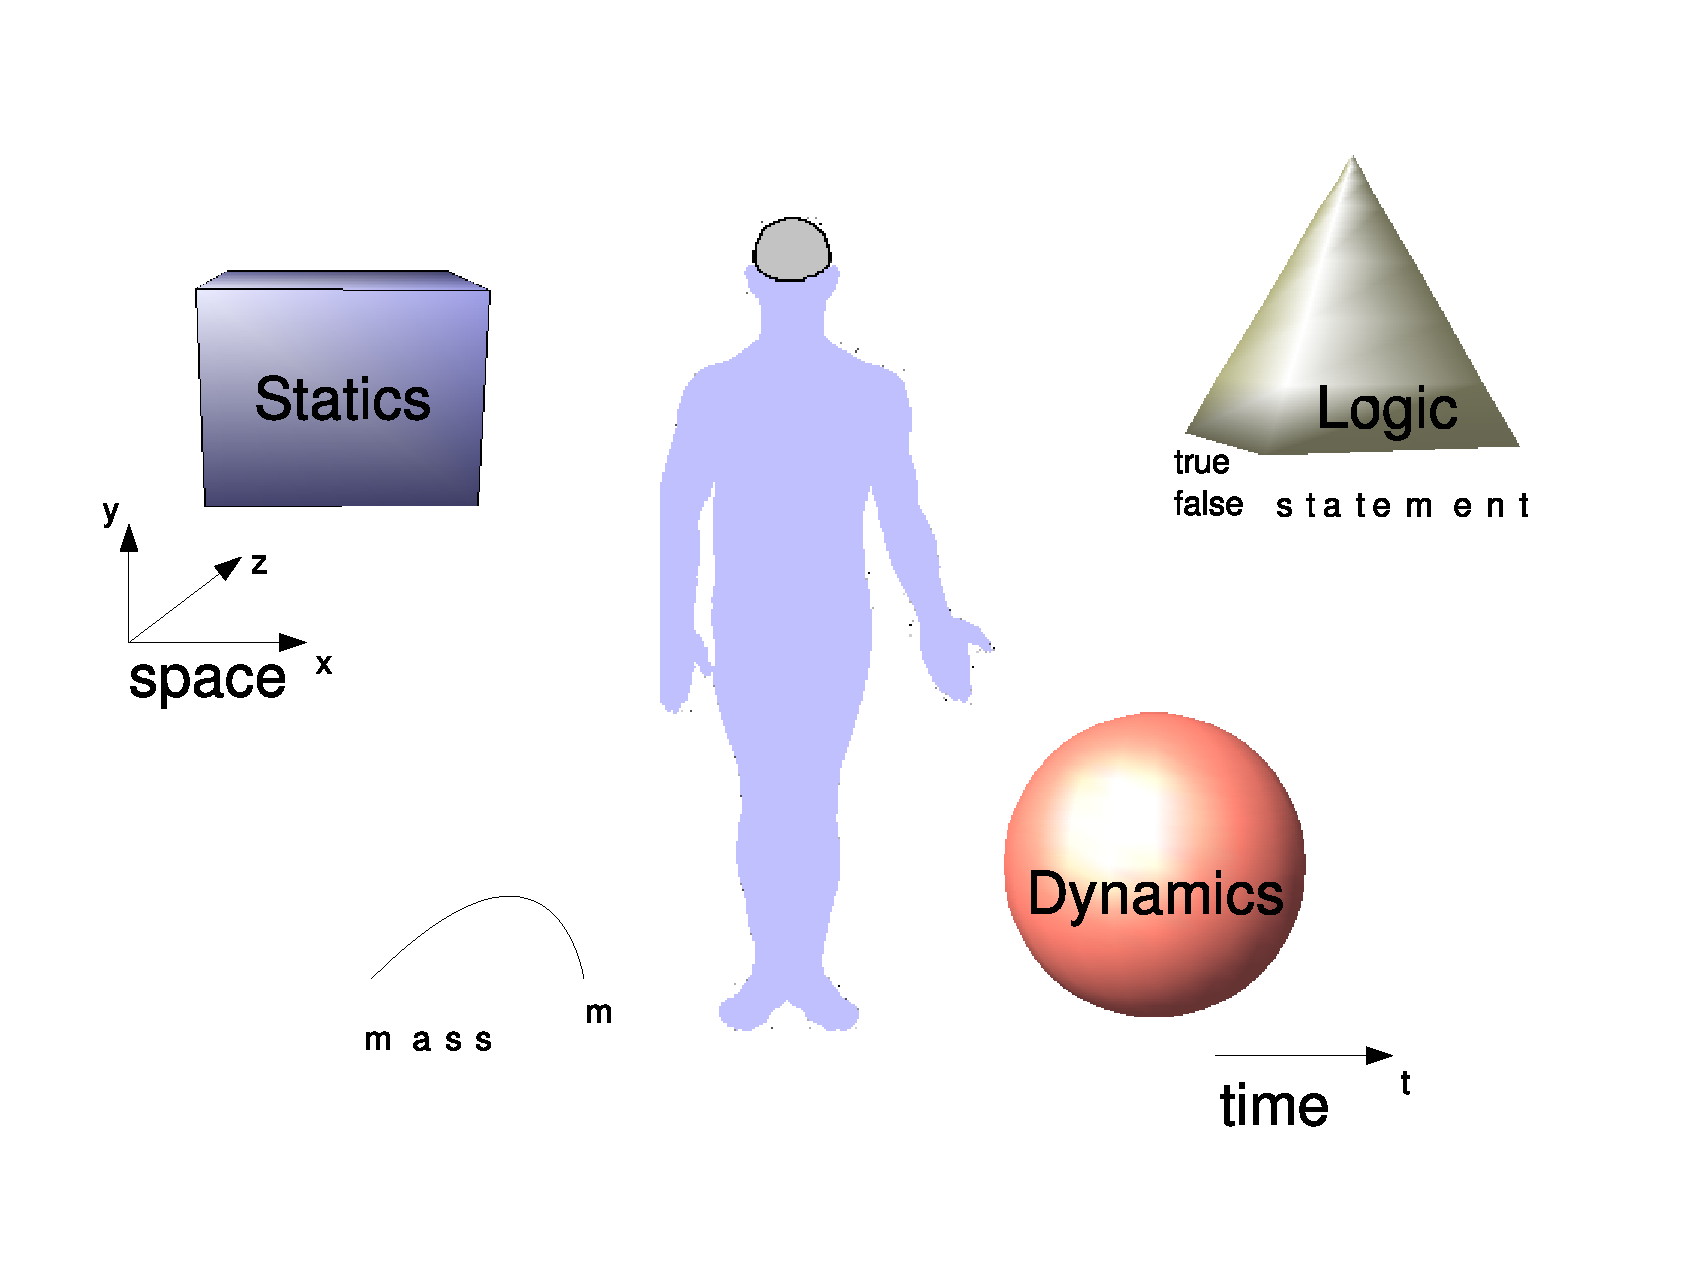
\includegraphics[scale=0.3]{vector/cybop.eps}
        \caption{CYBOP}
        \label{cybop_figure}
    \end{center}
\end{figure}

%
% $RCSfile: syntax.tex,v $
%
% Copyright (C) 2002-2008. Christian Heller.
%
% Permission is granted to copy, distribute and/or modify this document
% under the terms of the GNU Free Documentation License, Version 1.1 or
% any later version published by the Free Software Foundation; with no
% Invariant Sections, with no Front-Cover Texts and with no Back-Cover
% Texts. A copy of the license is included in the section entitled
% "GNU Free Documentation License".
%
% http://www.cybop.net
% - Cybernetics Oriented Programming -
%
% http://www.resmedicinae.org
% - Information in Medicine -
%
% Version: $Revision: 1.1 $ $Date: 2008-08-19 20:41:09 $ $Author: christian $
% Authors: Christian Heller <christian.heller@tuxtax.de>
%

\subsection{Syntax}
\label{syntax_heading}
\index{CYBOL Syntax}
\index{Syntax of a Language}
\index{Grammar of a Language}
\index{Extensible Markup Language}
\index{XML}
\index{XML Tag}
\index{XML Attribute}
\index{Discrimination}
\index{Composition}

Every language has a special \emph{Syntax}, that is a \emph{Grammar} with rules
for combining terms and symbols \cite{foldoc}. CYBOL could define its own
syntax or use an already existing one, of another language. Because of its
popularity, clear text representation, flexibility, extensibility and ease of
use, \emph{XML} was chosen to deliver the syntax for CYBOL.

To mention just two of the syntactical elements of XML, \emph{Tag} and
\emph{Attribute} are considered shortly here. Tags are special, arbitrary
keywords that have to be defined by the system working with an XML document.
Attributes keep additional information about the contents enclosed by two tags.
Two examples:

\begin{scriptsize}
    \begin{verbatim}
    <tag attribute="value">
        contents
    </tag>
    \end{verbatim}
\end{scriptsize}

\begin{scriptsize}
    \begin{verbatim}
    <tag attribute1="value" attribute2="contents"/>
    \end{verbatim}
\end{scriptsize}

An XML document carries a name and can such represent a \emph{Discrete Item},
as suggested by the principles of human thinking (section
\ref{human_thinking_heading}). Being a \emph{Compound}, it consists of parts --
and, it can link to other documents treated as its parts. That way, a whole
hierarchy can be formed. Tag attributes can keep additional information about
the linked parts. Most importantly, XML documents have a hierarchical structure
based on tags, which may be used to store meta information about a part.

Considering these properties of XML, it seems predestinated for formally
representing abstract models using the CYBOP concepts. CYBOL, finally, is XML
\emph{plus} a defined set of tags, attributes and values, used to structure and
link documents meaningfully.

%
% $RCSfile: vocabulary.tex,v $
%
% Copyright (C) 2002-2008. Christian Heller.
%
% Permission is granted to copy, distribute and/or modify this document
% under the terms of the GNU Free Documentation License, Version 1.1 or
% any later version published by the Free Software Foundation; with no
% Invariant Sections, with no Front-Cover Texts and with no Back-Cover
% Texts. A copy of the license is included in the section entitled
% "GNU Free Documentation License".
%
% http://www.cybop.net
% - Cybernetics Oriented Programming -
%
% http://www.resmedicinae.org
% - Information in Medicine -
%
% Version: $Revision: 1.1 $ $Date: 2008-08-19 20:41:09 $ $Author: christian $
% Authors: Christian Heller <christian.heller@tuxtax.de>
%

\subsection{Vocabulary}
\label{vocabulary_heading}
\index{CYBOL Vocabulary}
\index{Terms of a Language}
\index{Symbols of a Language}
\index{Syntax of a Language}
\index{Document Type Definition}
\index{DTD}
\index{XML Schema Definition}
\index{XSD}
\index{Extended Backus Naur Form}
\index{EBNF}

The \emph{Vocabulary} is what fills a language with life. It delivers the
\emph{Terms} and \emph{Symbols} that are combined after the rules of a syntax.

XML allows to define and exchange the whole vocabulary of a language. It offers
two ways in which a list of legal elements can be defined: The traditional
\emph{Document Type Definition} (DTD) and the more modern
\emph{XML Schema Definition} (XSD). Besides the vocabulary, DTD and XSD define
the structure of an XML document and allow to typify, constrain and validate
items. In addition to DTD and XSD, the \emph{Extended Backus Naur Form} (EBNF)
of CYBOL is given following.

The language definitions were not added as appendix to this work, because
firstly, they are not too long and secondly, an understanding of the CYBOL
elements is necessary to be able to grasp the constructs and examples given in
later sections.

%
% $RCSfile: document_type_definition.tex,v $
%
% Copyright (c) 2002-2007. Christian Heller. All rights reserved.
%
% Permission is granted to copy, distribute and/or modify this document
% under the terms of the GNU Free Documentation License, Version 1.1 or
% any later version published by the Free Software Foundation; with no
% Invariant Sections, with no Front-Cover Texts and with no Back-Cover
% Texts. A copy of the license is included in the section entitled
% "GNU Free Documentation License".
%
% http://www.cybop.net
% - Cybernetics Oriented Programming -
%
% Version: $Revision: 1.2 $ $Date: 2007-08-01 13:59:00 $ $Author: christian $
% Authors: Christian Heller <christian.heller@tuxtax.de>
%

\subsection{Document Type Definition}
\label{document_type_definition_heading}
\index{Document Type Definition}
\index{DTD}
\index{Extensible Markup Language}
\index{XML}
\index{Markup Tag}
\index{model Tag}
\index{part Tag}
\index{property Tag}
\index{constraint Tag}
\index{name Attribute}
\index{channel Attribute}
\index{abstraction Attribute}
\index{model Attribute}

A DTD represents the type definition of an XML document. It consists of a set
of \emph{Markup Tags} and their \emph{Interpretation} \cite{foldoc}. DTDs can
be declared inline, within a document, or as an external reference
\cite{w3schools}. Figure \ref{dtd_figure} shows the DTD of the CYBOL language.

\begin{figure}[ht]
    \bigskip
    \begin{scriptsize}
        \begin{verbatim}
<!ELEMENT model (part*)>
<!ELEMENT part (property*)>
<!ELEMENT property (constraint*)>
<!ELEMENT constraint EMPTY>

<!ATTLIST part
    name CDATA #REQUIRED
    channel CDATA #REQUIRED
    abstraction CDATA #REQUIRED
    model CDATA #REQUIRED>
<!ATTLIST property
    name CDATA #REQUIRED
    channel CDATA #REQUIRED
    abstraction CDATA #REQUIRED
    model CDATA #REQUIRED>
<!ATTLIST constraint
    name CDATA #REQUIRED
    channel CDATA #REQUIRED
    abstraction CDATA #REQUIRED
    model CDATA #REQUIRED>
        \end{verbatim}
    \end{scriptsize}
    \caption{Recommended CYBOL DTD}
    \label{dtd_figure}
\end{figure}

Following the pure hierarchical structure of CYBOL, it would actually suffice
to use a DTD as simple as the one shown in figure \ref{simpledtd_figure}. Since
the three elements \emph{part}, \emph{property} and \emph{constraint} (compare
figure \ref{dtd_figure}) have the same list of required attributes, they could
be summarised under the name \emph{part}, for example. Because the structure of
a CYBOL model is non-ambiguous, the meaning of its elements can be guessed from
their position within the model.

\begin{figure}[ht]
    \bigskip
    \begin{scriptsize}
        \begin{verbatim}
<!ELEMENT part (part*)>

<!ATTLIST part
    name CDATA #REQUIRED
    channel CDATA #REQUIRED
    abstraction CDATA #REQUIRED
    model CDATA #REQUIRED>
        \end{verbatim}
    \end{scriptsize}
    \caption{Simplified CYBOL DTD}
    \label{simpledtd_figure}
\end{figure}

\clearpage

For the purpose of expressing knowledge in accordance with the schema suggested
by CYBOP \cite{cybop}, a CYBOL knowledge template (file) does not need to have
a root element. The file name clearly identifies it. For reasons of XML
conformity, however, an extra root element called \emph{model} was defined
(figure \ref{dtd_figure}). And for reasons of better readability and
programmability, the three kinds of embedded elements were given distinct names.

\clearpage
%
% $RCSfile: xml_schema_definition.tex,v $
%
% Copyright (c) 2002-2007. Christian Heller. All rights reserved.
%
% Permission is granted to copy, distribute and/or modify this document
% under the terms of the GNU Free Documentation License, Version 1.1 or
% any later version published by the Free Software Foundation; with no
% Invariant Sections, with no Front-Cover Texts and with no Back-Cover
% Texts. A copy of the license is included in the section entitled
% "GNU Free Documentation License".
%
% http://www.cybop.net
% - Cybernetics Oriented Programming -
%
% Version: $Revision: 1.1 $ $Date: 2007-07-17 20:02:36 $ $Author: christian $
% Authors: Christian Heller <christian.heller@tuxtax.de>
%

\section{XML Schema Definition}
\label{xml_schema_definition_heading}
\index{XML Schema Definition}
\index{XSD}
\index{CYBOL XSD}
\index{XML Schema}
\index{Extensible Markup Language}
\index{XML}

\emph{XML Schema} is an XML-based alternative to DTD \cite{w3schools}, and XSD
is its definition language. There is a lot of discussion going on about the
sense or \emph{Myth} of XML Schema \cite{browne}, that this document will not
take part in. Figure \ref{xsd_figure} shows the XSD of the CYBOL language.

\begin{figure}[ht]
    \bigskip
    \bigskip
    \begin{scriptsize}
        \begin{verbatim}
<?xml version="1.0"?>
<xs:schema xmlns:xs='http://www.w3.org/2001/XMLSchema' targetNamespace='http://www.cybop.net'
    xmlns='http://www.cybop.net' elementFormDefault='qualified'>
    <xs:element name='part'>
        <xs:complexType>
            <xs:sequence>
                <xs:element ref='part' minOccurs='0' maxOccurs='unbounded'/>
            </xs:sequence>
            <xs:attribute name='name' type='xs:string' use='required'/>
            <xs:attribute name='channel' type='xs:string' use='required'/>
            <xs:attribute name='abstraction' type='xs:string' use='required'/>
            <xs:attribute name='model' type='xs:string' use='required'/>
        </xs:complexType>
    </xs:element>
</xs:schema>
        \end{verbatim}
    \end{scriptsize}
    \caption{Simplified CYBOL XSD}
    \label{simplexsd_figure}
\end{figure}

\begin{figure}[ht]
    \bigskip
    \bigskip
    \begin{scriptsize}
        \begin{verbatim}
<?xml version="1.0"?>
<xs:schema xmlns:xs='http://www.w3.org/2001/XMLSchema' targetNamespace='http://www.cybop.net'
    xmlns='http://www.cybop.net' elementFormDefault='qualified'>
    <xs:element name='model'>
        <xs:complexType>
            <xs:sequence>
                <xs:element ref='part' minOccurs='0' maxOccurs='unbounded'/>
            </xs:sequence>
        </xs:complexType>
    </xs:element>
    <xs:element name='part'>
        <xs:complexType>
            <xs:sequence>
                <xs:element ref='property' minOccurs='0' maxOccurs='unbounded'/>
            </xs:sequence>
            <xs:attribute name='name' type='xs:string' use='required'/>
            <xs:attribute name='channel' type='xs:string' use='required'/>
            <xs:attribute name='abstraction' type='xs:string' use='required'/>
            <xs:attribute name='model' type='xs:string' use='required'/>
        </xs:complexType>
    </xs:element>
    <xs:element name='property'>
        <xs:complexType>
            <xs:sequence>
                <xs:element ref='constraint' minOccurs='0' maxOccurs='unbounded'/>
            </xs:sequence>
            <xs:attribute name='name' type='xs:string' use='required'/>
            <xs:attribute name='channel' type='xs:string' use='required'/>
            <xs:attribute name='abstraction' type='xs:string' use='required'/>
            <xs:attribute name='model' type='xs:string' use='required'/>
        </xs:complexType>
    </xs:element>
    <xs:element name='constraint'>
        <xs:complexType>
            <xs:attribute name='name' type='xs:string' use='required'/>
            <xs:attribute name='channel' type='xs:string' use='required'/>
            <xs:attribute name='abstraction' type='xs:string' use='required'/>
            <xs:attribute name='model' type='xs:string' use='required'/>
        </xs:complexType>
    </xs:element>
</xs:schema>
        \end{verbatim}
    \end{scriptsize}
    \caption{Recommended CYBOL XSD}
    \label{xsd_figure}
\end{figure}

Again, a simplified version of that XSD could be created (figure
\ref{simplexsd_figure}). But for reasons explained before, the recommended XSD
is the one shown in figure \ref{xsd_figure}.

%
% $RCSfile: extended_backus_naur_form.tex,v $
%
% Copyright (C) 2002-2008. Christian Heller.
%
% Permission is granted to copy, distribute and/or modify this document
% under the terms of the GNU Free Documentation License, Version 1.1 or
% any later version published by the Free Software Foundation; with no
% Invariant Sections, with no Front-Cover Texts and with no Back-Cover
% Texts. A copy of the license is included in the section entitled
% "GNU Free Documentation License".
%
% http://www.cybop.net
% - Cybernetics Oriented Programming -
%
% http://www.resmedicinae.org
% - Information in Medicine -
%
% Version: $Revision: 1.1 $ $Date: 2008-08-19 20:41:06 $ $Author: christian $
% Authors: Christian Heller <christian.heller@tuxtax.de>
%

\subsubsection{Extended Backus Naur Form}
\label{extended_backus_naur_form_heading}
\index{Extended Backus Naur Form}
\index{EBNF}
\index{Backus Naur Form}
\index{BNF}
\index{CYBOL EBNF}

The EBNF adds regular expression syntax to the \emph{Backus Naur Form} (BNF)
notatation \cite{naur}, in order to allow very compact specifications
\cite{kuhn}. Figure \ref{ebnf_figure} shows the EBNF of the CYBOL language.

\begin{figure}[ht]
    \bigskip
    \bigskip
    \begin{scriptsize}
        \begin{verbatim}
CYBOL       = '<model>'
                    {part}
                '</model>';

part        = '<part ' attributes '\>' |
                '<part ' attributes '>'
                    {property}
                '</part>';

property    = '<property ' attributes '\>' |
                '<property ' attributes '>'
                    {constraint}
                '</property>';

constraint  = '<constraint ' attributes '\>';

attributes  = name_attribute channel_attribute abstraction_attribute model_attribute

name_attribute          = 'name="' name '"';
channel_attribute       = 'channel="' channel '"';
abstraction_attribute   = 'abstraction="' abstraction '"';
model_attribute         = 'model="' model '"';

name        = description_sign;
channel     = description_sign;
abstraction = description_sign;
model       = value_sign;

description_sign    = { ( letter | number ) };
value_sign          = { ( letter | number | other_sign ) };

letter          = small_letter | big_letter;
small_letter    = 'a' | 'b' | 'c' | 'd' | 'e' | 'f' | 'g' |
                    'h' | 'i' | 'j' | 'k' | 'l' | 'm' | 'n' |
                    'o' | 'p' | 'q' | 'r' | 's' | 't' | 'u' |
                    'v' | 'w' | 'x' | 'y' | 'z';
big_letter      = 'A' | 'B' | 'C' | 'D' | 'E' | 'F' | 'G' |
                    'H' | 'I' | 'J' | 'K' | 'L' | 'M' | 'N' |
                    'O' | 'P' | 'Q' | 'R' | 'S' | 'T' | 'U' |
                    'V' | 'W' | 'X' | 'Y' | 'Z';
other_sign      = ',' | '.' | '/', '+', '-', '*';
number          = '0' | '1' | '2' | '3' | '4' |
                    '5' | '6' | '7' | '8' | '9';
        \end{verbatim}
    \end{scriptsize}
    \caption{CYBOL in EBNF}
    \label{ebnf_figure}
\end{figure}

\clearpage

%\input{self_definition}
%Model and Metamodel \cite{sowa}, p. 431 and (for UML): p.436
%- UML needs a meta model describing its graphical model elements
%(Class, Association etc. are treated as classes themselves)
%- XML needs special definition languages (DTD, XSD)
%--> Show that CYBOL is its own meta model and can describe itself!

%
% $RCSfile: semantics.tex,v $
%
% Copyright (C) 2002-2008. Christian Heller.
%
% Permission is granted to copy, distribute and/or modify this document
% under the terms of the GNU Free Documentation License, Version 1.1 or
% any later version published by the Free Software Foundation; with no
% Invariant Sections, with no Front-Cover Texts and with no Back-Cover
% Texts. A copy of the license is included in the section entitled
% "GNU Free Documentation License".
%
% http://www.cybop.net
% - Cybernetics Oriented Programming -
%
% http://www.resmedicinae.org
% - Information in Medicine -
%
% Version: $Revision: 1.1 $ $Date: 2008-08-19 20:41:08 $ $Author: christian $
% Authors: Christian Heller <christian.heller@tuxtax.de>
%

\subsection{Semantics}
\label{semantics_heading}
\index{Semantics of a Language}
\index{CYBOL Semantics}
\index{State Knowledge Modelling}
\index{Logic Knowledge Modelling}
\index{Extensible Markup Language}
\index{XML}
\index{XML Tag}
\index{XML Attribute}

The meaning expressed by terms and sentences is their \emph{Semantics}
\cite{duden}.

CYBOL files can be used to model either \emph{State-} or \emph{Logic Knowledge}
(chapter \ref{state_and_logic_heading}). In both cases, the \emph{same} syntax
(document structure) with \emph{identical} vocabulary (XML tags and -attributes)
is applied. It is the attribute \emph{Values} that make a difference in meaning.

The double hierarchy proposed by CYBOP's knowledge schema (section
\ref{knowledge_representation_heading}) is put into static CYBOL knowledge
templates, by using XML \emph{Attributes} for representing the whole-part
hierarchy, and XML \emph{Tags} for representing the additional meta information
that a whole model keeps about its part models.

%
% $RCSfile: attributes.tex,v $
%
% Copyright (c) 2002-2007. Christian Heller. All rights reserved.
%
% Permission is granted to copy, distribute and/or modify this document
% under the terms of the GNU Free Documentation License, Version 1.1 or
% any later version published by the Free Software Foundation; with no
% Invariant Sections, with no Front-Cover Texts and with no Back-Cover
% Texts. A copy of the license is included in the section entitled
% "GNU Free Documentation License".
%
% http://www.cybop.net
% - Cybernetics Oriented Programming -
%
% Version: $Revision: 1.1 $ $Date: 2007-08-01 13:59:00 $ $Author: christian $
% Authors: Christian Heller <christian.heller@tuxtax.de>
%

\subsection{Attributes}
\label{attributes_heading}
\index{Attributes}
\index{name Attribute}
\index{channel Attribute}
\index{abstraction Attribute}
\index{model Attribute}

Normally, an XML \emph{Attribute} keeps meta information about the contents of
an XML \emph{Tag}. In CYBOL, however, three attributes keep meta information
about a fourth attribute. The attributes, altogether, are:

\begin{itemize}
    \item[-] name
    \item[-] channel
    \item[-] abstraction
    \item[-] model
\end{itemize}

The attribute of greatest interest is \emph{model}. It contains a model either
directly, or a path to one. The \emph{channel} attribute indicates whether the
\emph{model} attribute's value is to be read from:

\begin{itemize}
    \item[-] inline
    \item[-] file
\end{itemize}

The \emph{abstraction} attribute specifies how to interpret the model pointed
to by the \emph{model} attribute's value. A model may be given in formats like
for example:

\begin{itemize}
    \item[-] compound (a state- or logic compound model encoded in CYBOL format)
    \item[-] operation (a primitive logic model)
    \item[-] character
    \item[-] double
    \item[-] integer
    \item[-] boolean
\end{itemize}

The \emph{name} attribute, finally, provides the referenced model with an
identifier that has to be unique within the \emph{Whole} model the \emph{Part}
model belongs to.

While the interpretation of the \emph{model} attribute's value depends on the
\emph{channel-} and \emph{abstraction} attributes, the other three attributes
(\emph{name}, \emph{channel}, \emph{abstraction}) themselves always get
interpreted as string of characters.

%
% $RCSfile: tags.tex,v $
%
% Copyright (c) 2002-2007. Christian Heller. All rights reserved.
%
% Permission is granted to copy, distribute and/or modify this document
% under the terms of the GNU Free Documentation License, Version 1.1 or
% any later version published by the Free Software Foundation; with no
% Invariant Sections, with no Front-Cover Texts and with no Back-Cover
% Texts. A copy of the license is included in the section entitled
% "GNU Free Documentation License".
%
% http://www.cybop.net
% - Cybernetics Oriented Programming -
%
% Version: $Revision: 1.1 $ $Date: 2007-08-01 13:59:00 $ $Author: christian $
% Authors: Christian Heller <christian.heller@tuxtax.de>
%

\subsection{Tags}
\label{tags_heading}
\index{Tags}
\index{model Tag}
\index{part Tag}
\index{property Tag}
\index{constraint Tag}

There are many kinds of meta data besides the above-mentioned attributes, that
may be known about a model. These are given as special XML tags called
\emph{property} and \emph{constraint}. As defined in section
\ref{vocabulary_heading}, a CYBOL knowledge template may use four kinds of XML
tags:

\begin{itemize}
    \item[-] model
    \item[-] part
    \item[-] property
    \item[-] constraint
\end{itemize}

The \emph{model} tag appears just once. It is the root node which makes a CYBOL
knowledge template a valid XML document.

Of actual interest are the \emph{part} tags. They identify the models that the
\emph{whole} model described by the CYBOL knowledge template consists of.

A \emph{whole} model may know a lot more about its \emph{part} models, than is
given by a part model's XML attributes. A spatial state model may know about
the \emph{position} and \emph{size} of its parts, in space. A temporal model
(such as a workflow) may have to know about the \emph{position} of its parts in
time, in order to be able to execute them in the correct order. Further, the
temporal model needs to know about the \emph{input/output} (i/o) state models
which are to be manipulated by the corresponding logic operation (part model).
The number of parts within a whole (compound) model may be limited. And so on.
These additional information are provided by \emph{property} tags whose number
is conceptually unlimited.

Not only parts need additional meta data; properties may need such data, too.
The position or size as properties of a part may have to be constrained to
certain values, such as a \emph{minimum} or \emph{maximum}. The values of the
\emph{colour} property of a part model may have to be chosen out of a
pre-defined set called \emph{choice}. Data of that kind are stated in
\emph{constraint} tags.


%
% $RCSfile: example.tex,v $
%
% Copyright (c) 2001-2004. Christian Heller. All rights reserved.
%
% No copying, altering, distribution or any other actions concerning this
% document, except after explicit permission by the author!
% At some later point in time, this document is planned to be put under
% the GNU FDL license. For now, _everything_ is _restricted_ by the author.
%
% http://www.cybop.net
% - Cybernetics Oriented Programming -
%
% http://www.resmedicinae.org
% - Information in Medicine -
%
% @author Christian Heller <christian.heller@tuxtax.de>
%

\subsection{Example}
\label{example_heading}

The following example shows a minimalistic model of a (static) \emph{Graphical
User Interface} (GUI) frame.

\begin{verbatim}
<!--
    frame_example.cybol
/-->
<model>
    <part name="title"
        part_abstraction="string"
        part_model="Res Medicinae"/>
    <part name="menu_bar"
        part_abstraction="compound"
        part_model="/gui/menu_bar.cybol"
        position_abstraction="compass"
        position_model="north"/>
    <part name="status_bar"
        part_abstraction="compound"
        part_model="/gui/tool_bar.cybol"
        position_abstraction="compass"
        position_model="south"/>
</model>
\end{verbatim}

Similar models can be built of (dynamic) workflows whereby the inputs and outputs
of the part operations appear in a special order as attribute values. But this
may become the topic of a follow-up paper.

